\documentclass{standalone}
\usepackage{tikz} % Import the tikz package
\usetikzlibrary{automata} % Import library for drawing automata
\usetikzlibrary{positioning} % ...positioning nodes
\usetikzlibrary{arrows} % ...customizing arrows
\tikzset{node distance=2.5cm,
    every state/.style={
        semithick,
        fill=gray!10},
    initial text={},
    double distance=2pt,
    every edge/.style={
        draw,
        ->,>=stealth',
        auto,
        semithick}}
\let\epsilon\varepsilon
\begin{document}
    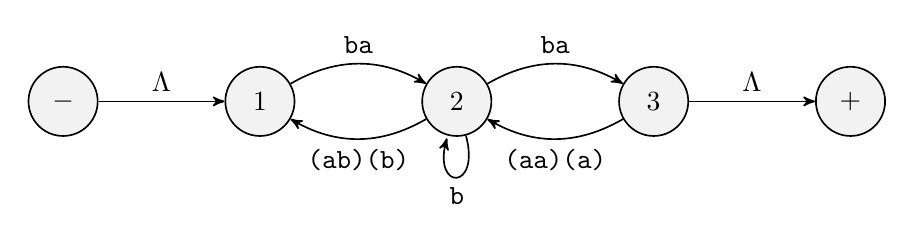
\begin{tikzpicture}
        \node[state] (mid) {$2$};
        \node[state,left of=mid] (ul) {$1$};
        \node[state,left of=ul] (start) {$-$};
        %\node[state, below left of=mid] (bl) {$4$};
        \node[state,right of=mid] (ur) {$3$};
        \node[state,right of=ur] (end) {$+$};
        %\node[state, below right of=mid] (br) {$5$};

        \draw (start) edge[] node {$\Lambda$} (ul); 
        \draw (ur) edge[] node {$\Lambda$} (end);
        \draw (ul) edge[bend left] node {\tt ba} (mid);
        %\draw (bl) edge[left] node {\tt b} (ul);
        \draw (mid) edge[bend left] node {\tt (ab)(b)} (ul);
        \draw (mid) edge[loop below] node {\tt b} (mid);
        \draw (mid) edge[bend left] node {\tt ba} (ur);
        %\draw (ur) edge[right] node {\tt aa} (br);
        \draw (ur) edge[bend left] node {\tt (aa)(a)} (mid);
    \end{tikzpicture}
\end{document}